% 
% Systemen voor Online Verkiezingen
% @author Pieter Maene <pieter.maene@student.kuleuven.be>
%

\documentclass[a4paper,journal]{IEEEtran}

% Hier kun je dan nog andere pakketten laden of eigen definities voorzien
\usepackage{amsmath,amssymb,mathtools}
\usepackage{enumitem}
\usepackage{float}
\usepackage[np,autolanguage]{numprint}
\usepackage{pdfpages}
\usepackage{subfig}
\usepackage{tikz}
\usepackage{url}

% De optie colorlinks mag verwijderd worden voor de af te drukken versie
\usepackage[pdfusetitle,plainpages=false]{hyperref}

% Customisations
\graphicspath{{./images/}}
\usetikzlibrary{arrows,fit,shapes}

% Document
\begin{document}

  %
% Alias
% @author Pieter Maene <pieter.maene@student.kuleuven.be>
%

\renewcommand{\ref}[1]{\mbox{\autoref{#1}}}

\renewcommand{\chapterautorefname}{Chapter}
\renewcommand{\equationautorefname}{Eq.}
\renewcommand{\figureautorefname}{Fig.}
\renewcommand{\footnoteautorefname}{Footnote}
\renewcommand{\itemautorefname}{Item}
\renewcommand{\sectionautorefname}{Section}
\renewcommand{\subsectionautorefname}{Section}
\renewcommand{\subsubsectionautorefname}{Section}
\renewcommand{\paragraphautorefname}{Paragraph}
\renewcommand{\subparagraphautorefname}{Paragraph}
\renewcommand{\pageautorefname}{Page}
\renewcommand{\tableautorefname}{Table}

\newcommand{\cplusplus}{C\texttt{++}\ }
  % 
% TikZ
% @author Pieter Maene <pieter.maene@student.kuleuven.be>
%

\tikzstyle{decision} = [diamond, draw, fill=black!20, text width=4.5em, text badly centered, node distance=3cm, inner sep=0pt]
\tikzstyle{block} = [rectangle, draw, fill=black!20, text width=5em, text centered, rounded corners, minimum height=4em]
\tikzstyle{line} = [draw, -latex']

  \title{Online Elections in Practice: Improvement and Application of the Helios Voting System}
  \author{Pieter~Maene}

  \maketitle
  
  \begin{abstract}    
    Helios is a voter-verifiable online voting system. Such a system allow the voter to verify whether his ballot was registered correctly and check the election result. The procedure for these systems is typically very complicated. The system's usability is determined by its interface which should support the procedure.
    
    \par This paper discusses the procedure to manage an election in Helios. The system's interface was modified to better support this procedure. The modified system is deployed for a real election where the election administrator and voters used it successfully. Additionally, the Web Cryptography API adds native cryptographic functionality to user agents. A benchmark showed that its implementation is faster, which could improve the usability of web applications.
  \end{abstract}
  
  % 
% Introduction
% @author Pieter Maene <pieter.maene@student.kuleuven.be>
%

\section{Introduction}



  % 
% Procedure
% @author Pieter Maene <pieter.maene@student.kuleuven.be>
%

\section{Procedure}
\label{sec:procedure}

This sections gives the procedure that should be followed to organise an election in the improved version of Helios (\ref{sec:user_interface_improvements}). Before he can start the procedure (\ref{sec:proc:helios}), the administrator should prepare some information (\ref{sec:proc:preparation}).

\subsection{Preparation}
\label{sec:proc:preparation}

%TODO Threshold scheme recommendation?

The trustees will be responsible for the decryption of the result. It is therefore important to give some thought to who this role will be given. Since using threshold encryption results in a more robust decryption process, it is advisable to use this. In that case, the election administrator should also determine the threshold scheme.

\par For each question, the number of answers that can be selected by the voter can be specified. The result for each answer can be shown either as the absolute number of votes it received, or its relative position with respect to the other answers.

\par Helios supports both open and closed elections. Anybody can vote in the former, while only specific voters are allowed to cast their ballot in the latter. A closed election should therefore be used when voter lists are available.

\subsection{Helios}
\label{sec:proc:helios}

The first step is the creation of the election. Here, all basic information like its name should be given. It is also possible to enable options here, like threshold encryption or whether the election is private or not. The start and end date of the election can be controlled here as well.

\par After creating the election, the trustees have to be added. This step was placed first in the procedure because it is the longest to complete. After being added, the trustee receives an e-mail with the link to his trustee dashboard.

\par If threshold encryption is not being used, each trustee simply has to generate a key pair. Once all trustees have done this, the election administrator can freeze the election. If threshold encryption was enabled, the key ceremony becomes more complicated. After adding all trustees, the election administrator can define the threshold scheme. The trustees can then start the following ceremony.

\begin{enumerate}
  \item The trustee has to generate his communication keys and upload the public keys to the server. They will be used to encrypt and sign the communication between them.
  \item Once all trustees have done this, each of them can generate his encrypted shares and send them to the others.
  \item After receiving a share from all other trustees, the trustee can decrypt and add them to obtain his share of the key that will be used to encrypt the ballots. It will serve as his private key for the election and he has to upload the corresponding public key.
\end{enumerate}

\par When all trustees have done this, the election can be frozen. Since the trustees will have to wait for the others, e-mails are sent to all of them when action is required.

\par Once the election is frozen, voters will be able to cast their ballot, unless a specific starting time was entered. If no end time was given, the election will be closed at the administrator's discretion.

\par After the election has been closed, the homomorphic tally can be decrypted. If threshold encryption is not enabled, all trustees will have to calculate their decryption factor and submit it. Otherwise, only the number of trustees defined in the threshold scheme will have to do this.

  % 
% Interface
% @author Pieter Maene <pieter.maene@student.kuleuven.be>
%

\section{User Interface Improvements}
\label{sec:user_interface_improvements}

Most of our work on the interface to improve the usability concentrated on two big parts of Helios. First, the admin was modified to better reflect the procedure discussed in \ref{sec:procedure}. This was done by creating a separate admin page where the procedure is clearly shown to the election administrator. Second, the trustee dashboard was also simplified. Here, the HTML5 File API was used to make it easier for the trustee to manage his keys. Additionally, the layout was streamlined throughout the application. 

\subsection{Admin}

The original interface integrated the administrative functions in the election view. This made it hard for the election admin to keep track of his progress in the procedure. It was therefore decided to move this functionality to a separate page. It shows the entire procedure and clearly indicates which steps have been completed. Since the actions lead away from this page, a bar was put on top of all pages where the progress is indicated as well.

\par The workflow for an election with threshold encryption is thoroughly changed. Originally, a public bulletin board was available where anybody could upload a pair of communication keys. The admin could only add trustees to an election from a list of people who had done this. This meant that he had to wait for all trustees to do this before he could define the threshold scheme and continue setting up the election. This required a secondary path of communication, outside of Helios. Because the bulletin board was publicly accessible, an attacker could impersonate a trustee. Unless he has access to the trustee's e-mail account, he would not receive the URL to the trustee dashboard. In that case, he would only have been able to stall the key ceremony.

\par The bulletin board was removed completely and trustees are immediately added to the election. They then receive an e-mail with a unique link to their trustee dashboard where they generate their communication keys.

\subsection{Trustee Dashboard}

The trustees will perform all actions of the key ceremony in the trustee dashboard. The trustee's role is explained and an overview of all steps in the ceremony is shown in the same way as the election procedure on the admin page.

\par The trustee will generate three key pairs during the ceremony. The private keys are stored locally in JSON files. Originally, the JSON was simply shown to the user and he had to manually save it to a file. When the key was needed, the file's contents needed to be copied again to a text area.

\par The HTML5 File API offers two API interfaces that can be used to ease this process.\cite{ranganathan_sicking_file_api} The first is the \texttt{Blob} interface that can be used to generate files in JavaScript. They can then be offered as a download in the browser. The second is the \texttt{FileReader} interface which allows a web developer to read files that conform to the \texttt{Blob} or \texttt{File} interfaces.

\par They are used in the trustee dashboard to offer the secret keys as a download. The details of the key are now hidden from the trustee. When his key is needed, he has to select this file in an input element. The file's contents are then read to the text area. These adjustments make it a lot easier for the trustee to manage his keys.

\par In addition to using this API, the two secret keys of the communication pair are now stored in a single file. Since the distinction between two was only confusing to the trustee, this simplifies the key management for him.

\subsection{Voting Booth}

The tests that were performed before using Helios for the real election will be discussed in \ref{sec:be:tests}. The voting booth is simplified based on feedback that was received during the test of the voting booth. The changes that were made will be detailed in that section.

  % 
% Application
% @author Pieter Maene <pieter.maene@student.kuleuven.be>
%

\section{Board Election}
\label{sec:board_election}

The modified Helios voting system was used in the elections for the new board of VTK, the official student organisation for engineering students at the KU Leuven. Support for some specific features was added. The system was then thoroughly tested before the election on May 8\textsuperscript{th} 2014.

\subsection{Election Requirements}

%TODO Election Requirements

A committee of at least five people from the current board watches over the election. The head of this committee is the current president of the board. He should be able to manage the election. It should be possible to appoint the other members as trustees. The decryption process cannot be blocked by one trustee.

%TODO Herschrijven

\par There are two types of candidates: the first can be officially elected as the next board, the second participates for fun. Both should be separate questions on the ballot. If there is only one official team, voters have to be able to vote pro or contra, or to abstain. If there are two teams, at most one should be selectable. If there are more than two, voters should express their appreciation for each team. However, this last case is so rare that it's not a strong requirement for the system. In the election of the fun team, it should be possible to select all of them at most.

\par A list of all eligible voters can be requested from the university. These lists bear the student's first name, last name and university identification number. Only these voters should be able to access the election. Therefore, an authentication system should be available. Finally, the participation percentage should be shown on the result page.

\subsection{Specific Adjustments}

Shibboleth is the single sign-on system used by the KU Leuven. Students have an account with a unique identification number. All voters in the election have such an account, so it could be used to authenticate them. Since Helios' authentication system is modular and already has support for other federated identity systems, adding Shibboleth was relatively straightforward.

\par The list of voters was provided by an external organisation. This included the student's identification number and name, but the e-mail address was missing. This is needed by Helios to send a confirmation message after casting a ballot. A voter's e-mail address is retrieved from the Shibboleth response and added to the account to fix this.

\par Helios did not yet show the election's participation percentage. This is the percentage of eligible voters that cast their vote. The system also immediately published the election result. These are traditionally announced to the public at midnight, but the election administrator does need earlier access. These two smaller features were therefore implemented as well.

\subsection{Tests}
\label{sec:be:tests}

After installing the system on a server, it was thoroughly tested by the current board of VTK. In addition to verifying all technical aspects, the testers were also asked for feedback on the user interfaces. The election admin and booth were tested in the context of the actual election. The real voter list was replaced by the current board of the organisation, though.

\par While testing the threshold encryption process, a bug was found. Real fractions were used for the calculation of the Lagrange interpolation, instead of finite modular arithmetic. After solving this, the result still couldn't be decrypted correctly. By default, Helios was added as a trustee to the election. It completed all steps in the ceremony automatically. During testing, the shares of this trustee turned out to be incompatible with these generated by the other trustees. The only difference between the two is that the former are generated in the Python application and the latter in the JavaScript trustee dashboard. Because the source of the error origin could not be found, Helios no longer could be an election trustee. Since its role in the whole process was already limited, this was not a major change. The main advantage of adding it, was that it allowed users to create an election without real trustees, which resulted in a simpler procedure.

\par Apart from these bugs, the test of the election admin went very well. The election administrator managed to go through the entire procedure independently. The trustees didn't have much difficulty generating their keys either.

\par Although its functionality worked perfectly, a lot of feedback was given on the voting booth. First, a lot of technical terms were used. This was easily solved by replacing them with more common words. Second, most testers found the voting process to be too complicated. The booth is an independent application written in JavaScript, so that only the encrypted vote is sent to the server.

\par There were two places where the user had to submit his vote originally (\ref{fig:be:voting_booth_flows}). After confirming his encrypted vote in the booth, it was sent to the server where it could finally be cast. The last screen of the voting booth was therefore removed. Since it still had to be possible to audit the encrypted vote, this also required the encryption to be moved. This is now done after the voter has made all his choices. As a result, the vote has to be encrypted again when these are changed. The current implementation is already reasonably fast and this will only improve once the Web Cryptography API is available (\ref{sec:web_cryptography_api}). Finally, an alert is shown when voters try to leave the page where they have to upload their ballot to the server before doing so. The test was repeated after making these adjustments to verify their impact on both functionality and usability.
 
\begin{figure}
  \centering
  \begin{minipage}{.45\linewidth}
    \centering
    \scalebox{.6}{\begin{tikzpicture}[node distance=2cm, auto]
  \node [block] (intro) {Introduction};
  \node [block, below of=intro] (select) {Select Choices};
  \node [block, below of=select] (review) {Review Choices};
  \node [decision, below of=review] (decide) {Satisfied with Choices?};
  \node [block, below of=decide, node distance=3cm] (confirm) {Confirm Ballot};
  \node [block, below of=confirm, node distance=2.5cm] (submit) {Submit Ballot};
  \node [block, below of=submit] (cast_confirm) {Submission Confirmation};

  \path [line] (intro) -- (select);
  \path [line] (select) -- (review);
  \path [line] (review) -- (decide);
  \path [line, dashed] (decide) -- node(encrypt){Encrypt Ballot} (confirm);
  \path [line, dashed] (confirm) -- node{Leave Voting Booth} (submit);
  \path [line] (submit) -- (cast_confirm);
  
  \draw [line] (decide.west) -- node{No} ++(-1.5,0) node(lower_right){} |- (select.west);
  \draw [line] (confirm.east) -- node{Audit} ++(1.75,0) node(lower_left){} |- (encrypt.east);
\end{tikzpicture}}
  \end{minipage}
  \quad
  \begin{minipage}{.45\linewidth}
    \centering
    \scalebox{.6}{\begin{tikzpicture}[node distance = 2cm, auto]
  \node [block] (intro) {Introduction};
  \node [block, below of=intro] (select) {Select Choices};
  \node [block, below of=select, node distance=2.5cm] (review) {Review Choices};
  \node [decision, below of=review] (decide) {Satisfied with Choices?};
  \node [block, below of=decide, node distance=3cm] (submit) {Submit Ballot};
  \node [block, below of=submit] (cast_confirm) {Submission Confirmation};

  \path [line] (intro) -- (select);
  \path [line, dashed] (select) -- node(encrypt){Encrypt Ballot} (review);
  \path [line] (review) -- (decide);
  \path [line, dashed] (decide) -- node{Leave Voting Booth} (submit);
  \path [line] (submit) -- (cast_confirm);
  
  \draw [line] (decide.west) -- node{No} ++(-1.5,0) node(lower_left){} |- (select.west);
  \draw [line] (decide.east) -- node{Audit} ++(1.5,0) node(lower_right){} |- (encrypt.east);
\end{tikzpicture}}
  \end{minipage}
  \caption{Old (Left) and New (Right) Voting Booth Flows}
  \label{fig:be:voting_booth_flows}
\end{figure}

\par Finally, a stress test was run as well. This was done for a separate election with two trustees and three questions. \np{1000} votes were inserted into the database. To do this, the encrypted votes were generated directly in Python instead of using the JavaScript voting booth. The result was decrypted successfully, indicating that the system can manage an election of that size.

\subsection{Election Day}

The election itself took place on May 8\textsuperscript{th} 2014 from 7 am till 8 pm. During this time, 768 people cast a ballot, which isn't significantly less than during previous years. This is a strong indication that the voting process was clear. No complaints were received from these voters either.

\par Since everything had been tested in advance, no problems were encountered during the voting or when decrypting the result.

  % 
% Web Cryptography API
% @author Pieter Maene <pieter.maene@student.kuleuven.be>
%

\section{Web Cryptography API}
\label{sec:web_cryptography_api}

Currently, web developers implement cryptographic functionality in JavaScript. Despite great improvements in recent years, it is still slower than native code.\cite{site:resig_javascript_performance_rundown}\cite{site:cois_javascript_performance_rundown_2012}\cite{smedberg_performance_analysis_of_javascript} In 2012 a working group was started by W3C to write the Web Cryptography API specification, which would add cryptographic functionality to user agents.\cite{wiki:webcrypto} The specification defines the \texttt{SubtleCrypto} interface which has several high-level functions.\cite{sleevi_watson_web_cryptography_api} There are methods to manage the keys and to encrypt data. The API only supports a specific set of algorithms, nor does each algorithm support all functions of the interface.

\par Since the specification has not been completed yet, most user agents do not support it. Internet Explorer 11 is the only browser that already has an implementation, but it misses some algorithms.\cite{site:microsoft_web_cryptography} Therefore, the NfWebCrypto polyfill was used for the benchmarks. This is a \cplusplus plugin for Chrome, so its performance should be comparable to a real implementation.

\subsection{Modular Exponentation}
\label{sec:wc:modular_exponentiation}

Helios uses ElGamal to encrypt the ballots, which is an algorithm not supported by the API. The modular exponentiations are responsible for the majority of the calculation time. An improvement there would impact overall performance.

\par Since the API only offers high-level functions, this had to be implemented separately. Diffie-Hellman is one of the supported algorithms. The \texttt{deriveKey} method uses \ref{eq:wc:diffie_hellman} to calculate the shared secret.\cite{diffie_hellman_new_directions_in_cryptography}

\begin{equation}
  \label{eq:wc:diffie_hellman}
  K = (g^a)^b \mod{p}
\end{equation}

\par In this equation, $g^a$ is the public key of A and $b$ the private key of B. If the public and private key can be specified, it can be used to calculate the modular exponentiation $x^y \mod{p}$. It is possible to import a specific private key into the user agent's key store. For the Diffie-Hellman algorithm, the specification only allows private keys in the PCKS8 format to be imported. To make testing easier, the NfWebCrypto plugin was modified to allow the import of raw keys. After calculating the shared secret, the result can be obtained with the \texttt{exportKey} function.

\par The performance of the NfWebCrypto library is compared to that of JSBN and Leemon, two JavaScript big number libraries.\cite{site:wu_rsa_and_ecc_in_javascript}\cite{site:baird_big_integers_in_javascript} A \np{1024}-bit exponent is used, which is the size of the keys used by Helios. The calculation is repeated \np{1000} times for each library. The results are shown in \ref{fig:wc:modular_exponentiation} and \ref{tab:wc:modular_exponentiation}. The first exponentiation of the NfWebCrypto plugin took a lot longer, which explains the large variance. The NfWebCrypto plugin result was not correct. The communication with the plugin has to be \texttt{base64} encoded, which resulted in conversion issues between \cplusplus and JavaScript.

\begin{figure}
  \center{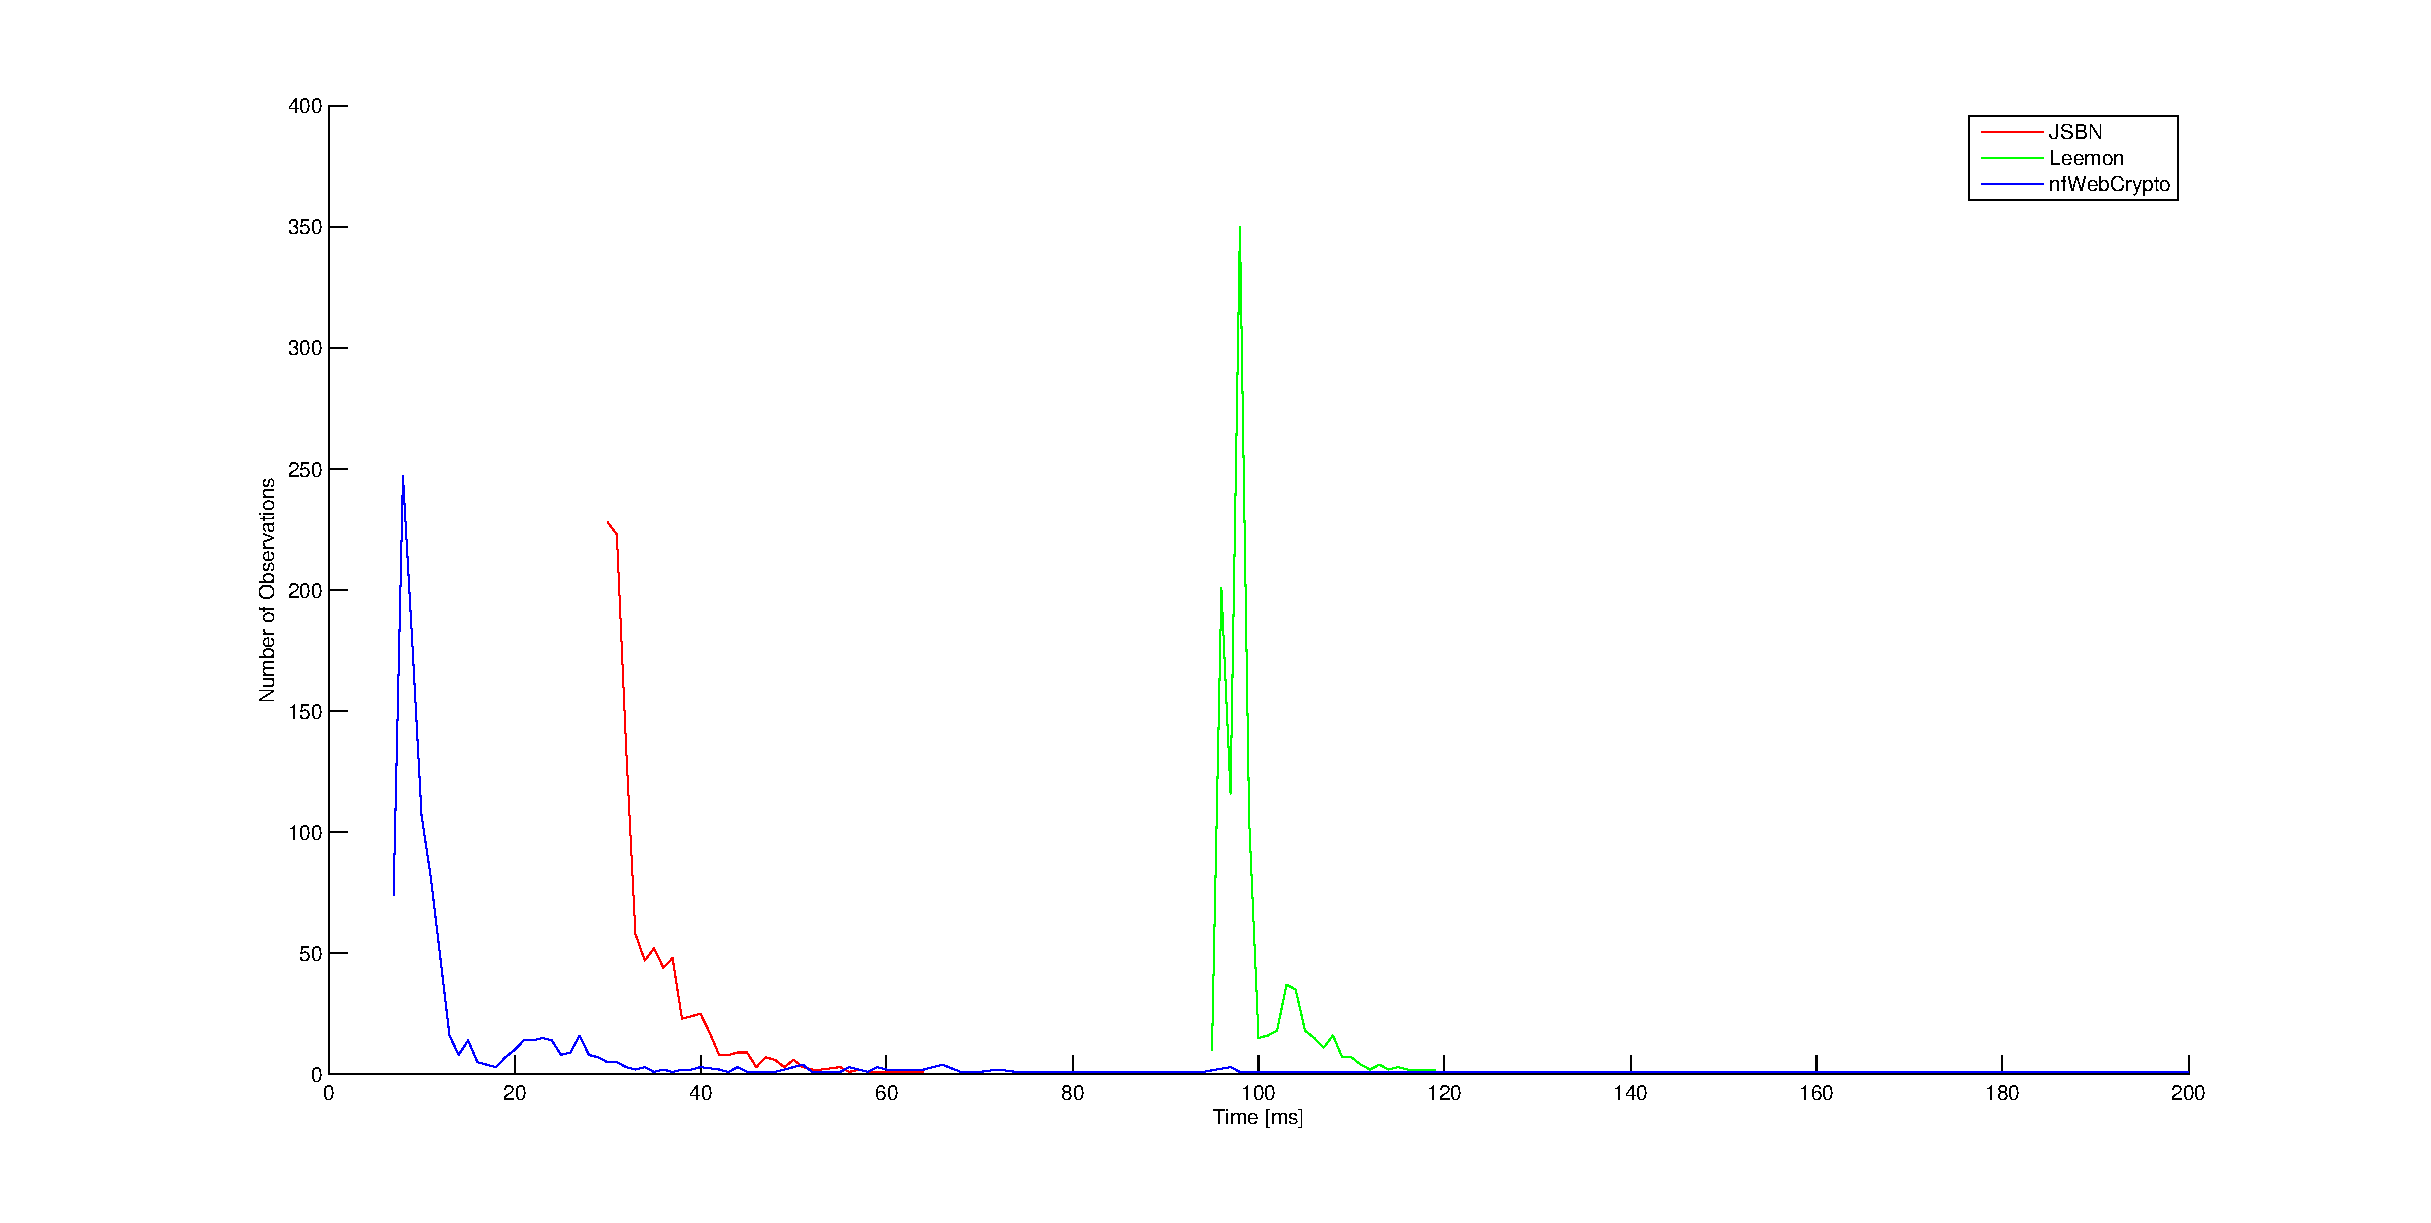
\includegraphics[width=\linewidth]{modular_exponentiation.eps}}
  \caption{Modular Exponentiation}
  \label{fig:wc:modular_exponentiation}
\end{figure}

\begin{table}
  \begin{center}
    \begin{tabular}{r | c c}
      Library & Gemiddelde [ms] & Variantie [ms] \\ \hline
      JSBN & 33,9250 & 26,5019  \\
      Leemon & 99,1470 & 15,0785 \\
      NfWebCrypto & 16,0670 & 470,6251
    \end{tabular}
    \caption{Modular Exponentiation}
    \label{tab:wc:modular_exponentiation}
  \end{center}
\end{table}

\subsection{RSA}

RSA was used to make a second comparison between JSBN and NfWebCrypto. This cipher isn't used by Helios, but the results are very interesting. A standard value of \np{65537} was used for the public exponent of the encryption. Notice that this is a lot shorter than the exponents used in \ref{sec:wc:modular_exponentiation}. The modulus is \np{1024} bits large.

\par JSBN has specific functions for RSA encryption and decryption. The Web Cryptography API supports the \texttt{RSAES-PKCS1-v1\_5} algorithm.\cite{rfc3447} Although public keys in the SPKI format can be imported, this proved difficult. Therefore, a new key was generated for each encryption. The time required for this is not taken into account. The results are shown in \ref{fig:wc:rsa} and \ref{tab:wc:rsa}. Surprisingly, the JavaScript implementation is faster than the NfWebCrypto plugin. This is caused by communication overhead.

\begin{figure}
  \center{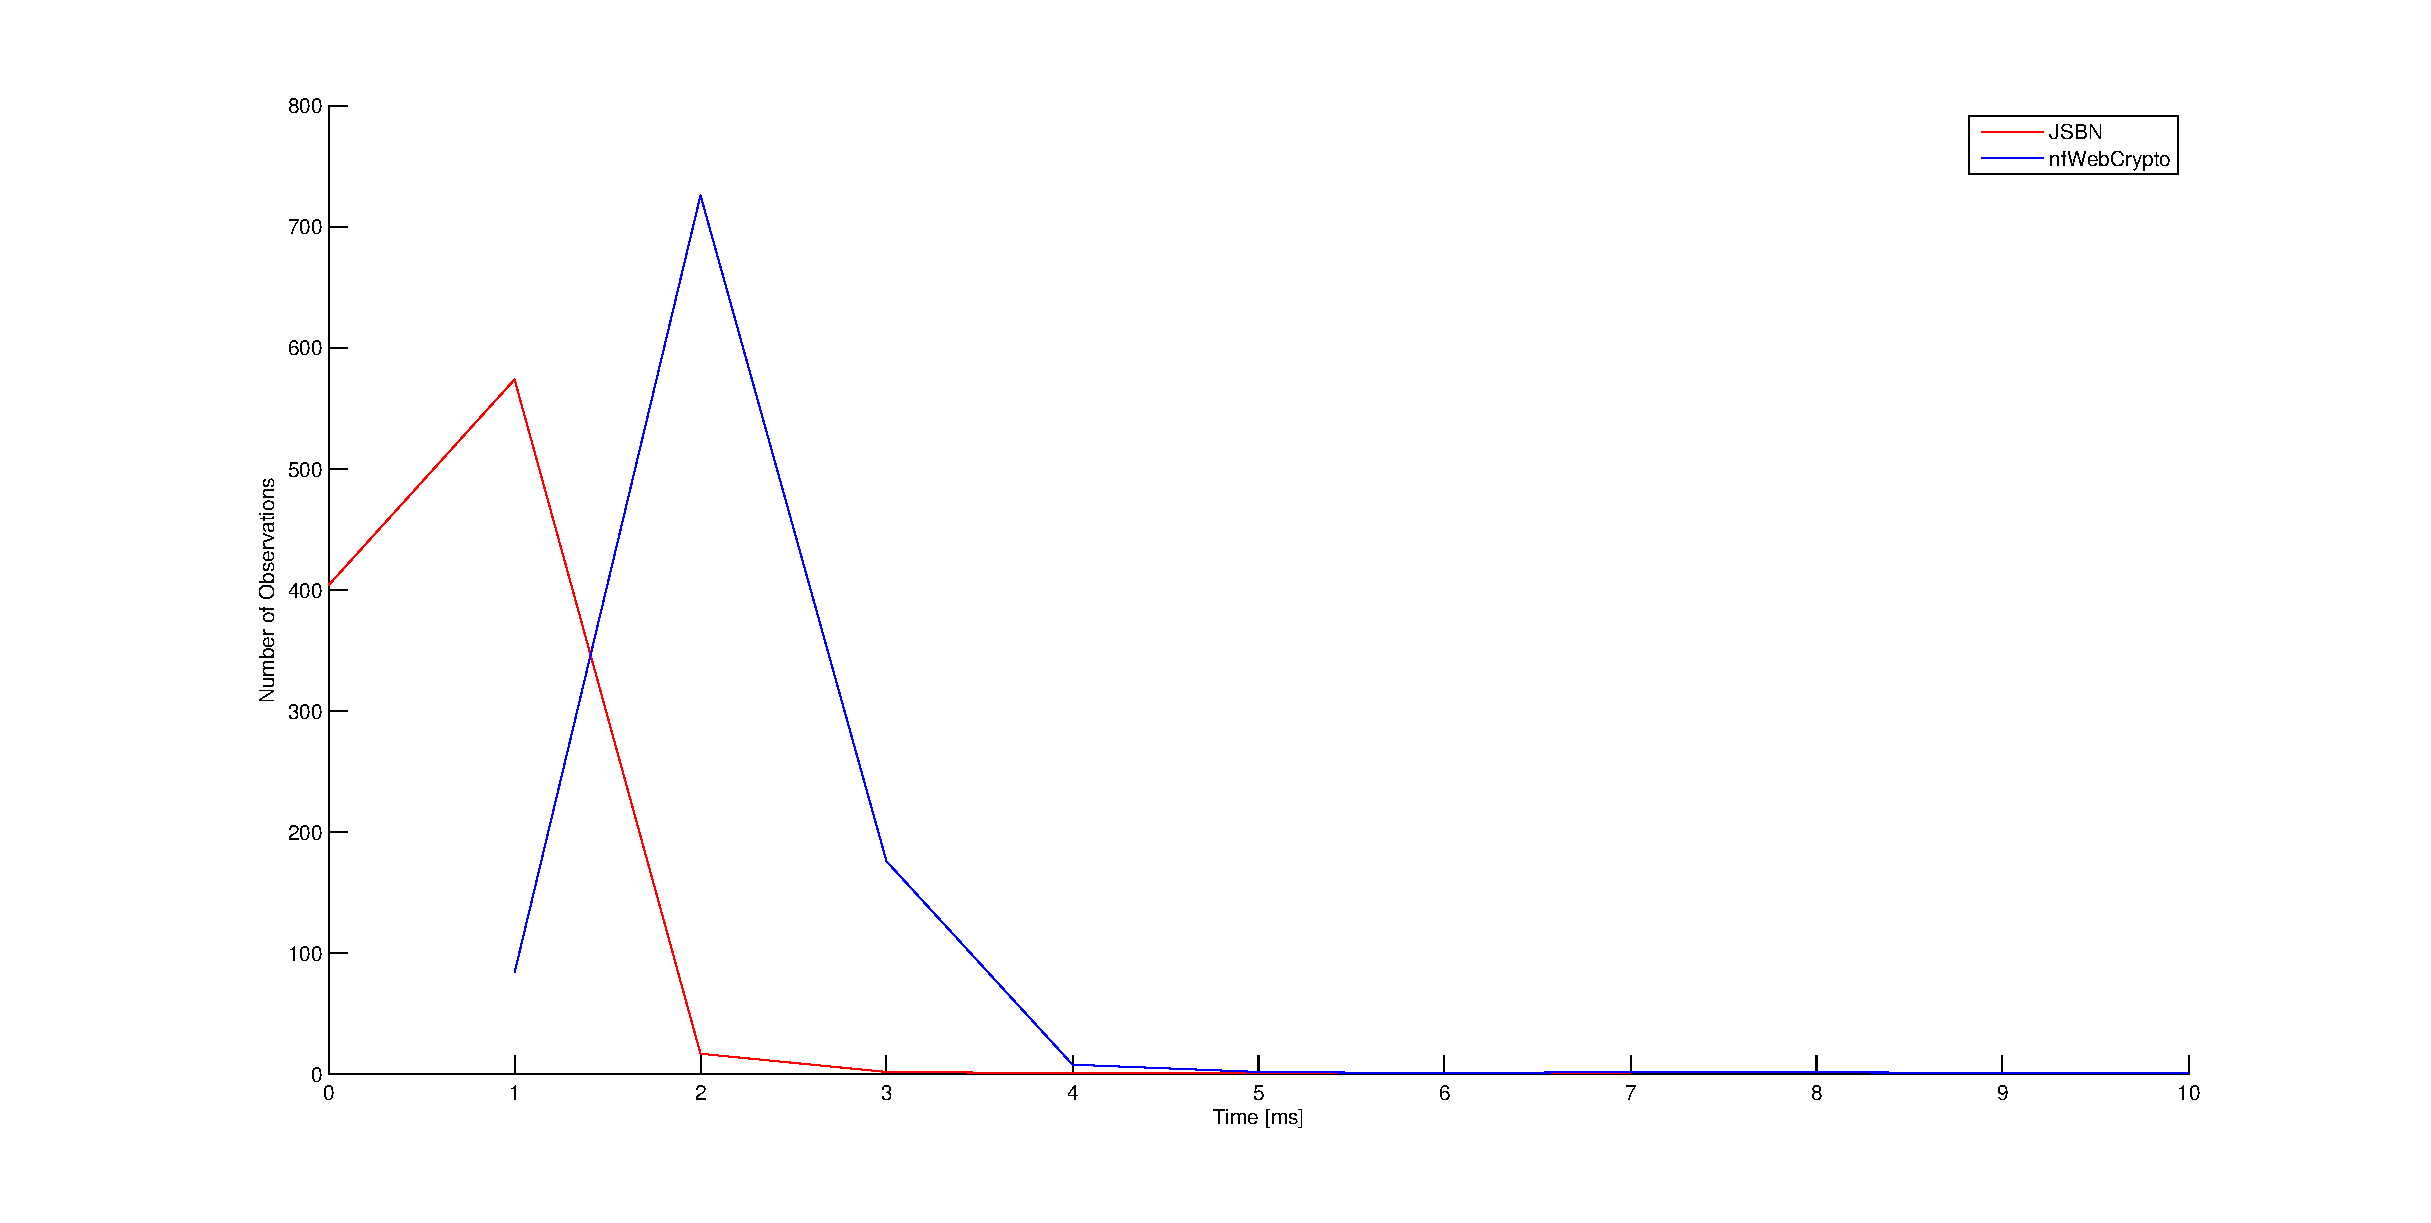
\includegraphics[width=\linewidth]{rsa.eps}}
  \caption{RSA}
  \label{fig:wc:rsa}
\end{figure}

\begin{table}
  \begin{center}
    \begin{tabular}{r | c c}
      Library & Gemiddelde [ms] & Variantie [ms] \\ \hline
      JSBN & 0,6310 & 0,3632  \\
      NfWebCrypto & 2,1360 & 0,4219
    \end{tabular}
    \caption{RSA}
    \label{tab:wc:rsa}
  \end{center}
\end{table}

  % 
% Conclusion
% @author Pieter Maene <pieter.maene@student.kuleuven.be>
%

\section{Conclusion}
  
  \bibliographystyle{IEEEtran}
  \bibliography{references}

  \begin{IEEEbiography}[{\includegraphics[width=1in,height=1.25in,clip,keepaspectratio]{pieter_maene.jpg}}]{Pieter Maene} was born in Duffel in the year 1991. Because of an interest in science and technology, he started engineering studies at the KU Leuven in 2009. He enrolled in the electrical engineering master in 2011 where he took courses on signal processing, embedded systems and cryptography.
  \end{IEEEbiography}

\end{document}
